\documentclass{article}
\usepackage{pgfplots}
\begin{document}
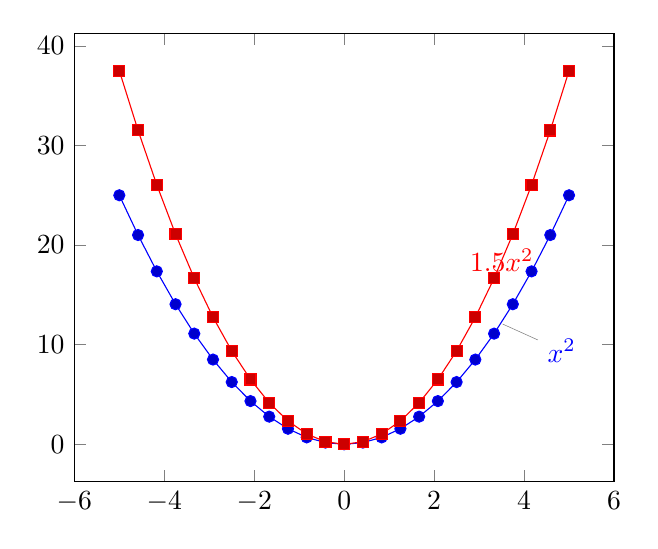
\begin{tikzpicture}
  \begin{axis}
    \addplot {x^2} node [pos=0.75,pin={-10:$x^2$},inner sep=0pt] {}; % This does not position the node on the line
    \addplot {1.5*x^2} node [pos=0.75] {$1.5x^2$};
    %% \node at (axis cs:4,16) [pin={-10:$x^2$},inner sep=0pt] {}; % This is what I want, but without calculating the coordinates by hand
    %% \node at (axis cs:4,24) [pin={170:$1.5 x^2$},inner sep=0pt] {};

  \end{axis}
\end{tikzpicture}
    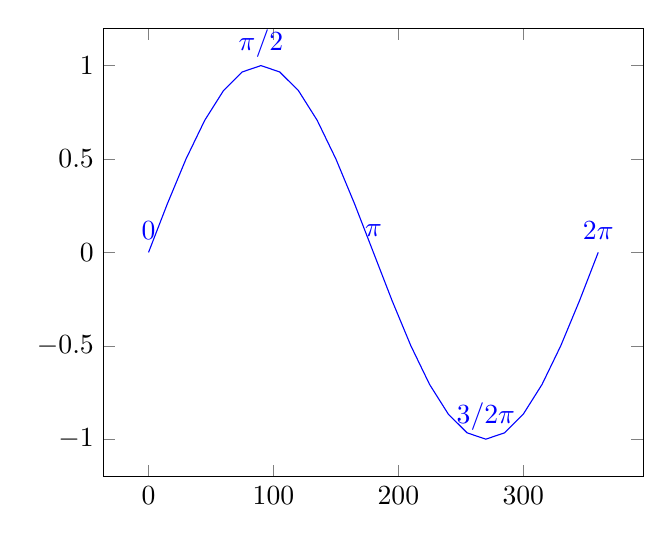
\begin{tikzpicture}
      \begin{axis}
        \addplot[blue,domain=0:360] {sin(x)}
                [yshift=8pt]
                node[pos=0] {$0$}
                node[pos=0.25] {$\pi/2$}
                node[pos=0.5] {$\pi$}
                node[pos=0.75] {$3/2\pi$}
                node[pos=1] {$2\pi$};
      \end{axis}
      \end{tikzpicture}
\end{document}
